%%%%%%%%%%%%%%%%%%%%%%%%%%%%
%%%%%%%%%%%%%%%%%%%%%%%%%%%%
\section{Detection of conflicting phylogenetic signals} \label{sec:extensions}

The very idea of a consensus tree relies on the existante of a \emph{center} around which trees are distributed. However, trees that are far away from the consensus can be the sign of either high variability or conflicting signals. While high variability implies weak phylogenetic signal, conflicting  signals implies incongruence in the underlying data. Most distances, such as RF, are discrete and lead to very coarse information about the tree distribution. By contrast, continuous distances are a natural way to characterize variance and distinguish high variability from conflicting signals. Moreover continuous distance lend themselves nicely to other standard aspects of inferential statistics such as confidence sets and hypothesis testing.

%Consider the space tree
%\begin{itemize}
% \item BHV space topology
% \item Means and variances in the tree space \textcolor{red}{briefly mentioned in previous section}
% \item Multivariate Analysis based on tree distances
% \end{itemize}

The  geometric  model of \citet{Billera2001} allows one to compare phylogenetic trees with the same taxa set (of size $m$) in a quantitative way. This  space  has  a  natural  metric, giving a way of measuring \emph{continuous} distances between phylogenies and providing some procedures for averaging or combining several trees with the same leaves. This geometry also shows which trees appear within a fixed distance of a given tree and enables one to build confidence convex hulls from a set of trees. It also provides a justification for calling outliers in a collection of otherwise congruent trees and limit the consensus to those congruent tree.

%%%%%%%%%%%%%%%%%%%%%%%%%%%%
\subsection{Tree Space definition} \label{sec:Tree-distances}
 The distance $d(T,T')$ between two trees $T$ and $T'$ accounts for differences with respect to both their tree topologies (branching structure) and branch lengths. The space is constructed by representing each of the $(2m-3)!!$ possible tree topologies by a single non-negative Euclidean orthant of dimension $m-3$ (the largest possible number of internal branches). The orthants are then “glued together” along appropriate axes. Specifically, nearest neighbor interchange (NNI) topologies lie in adjacent non-negative orthants along the boundary corresponding to the collapse of the relevant NNI edge.

For two trees with different topologies, the BHV distance is the length of the shortest path that link them in the treespace. The length of any path can be computed by calculating the Euclidean distance of the path restricted to each orthant that it passes though, and summing these lengths. The shortest path is called a geodesic, and will pass from one orthant to the next orthant through lower-dimensional boundaries corresponding to less resolved trees. Since the space is nonpositively  curved, the geodesics are unique.

\begin{figure}
\centering
 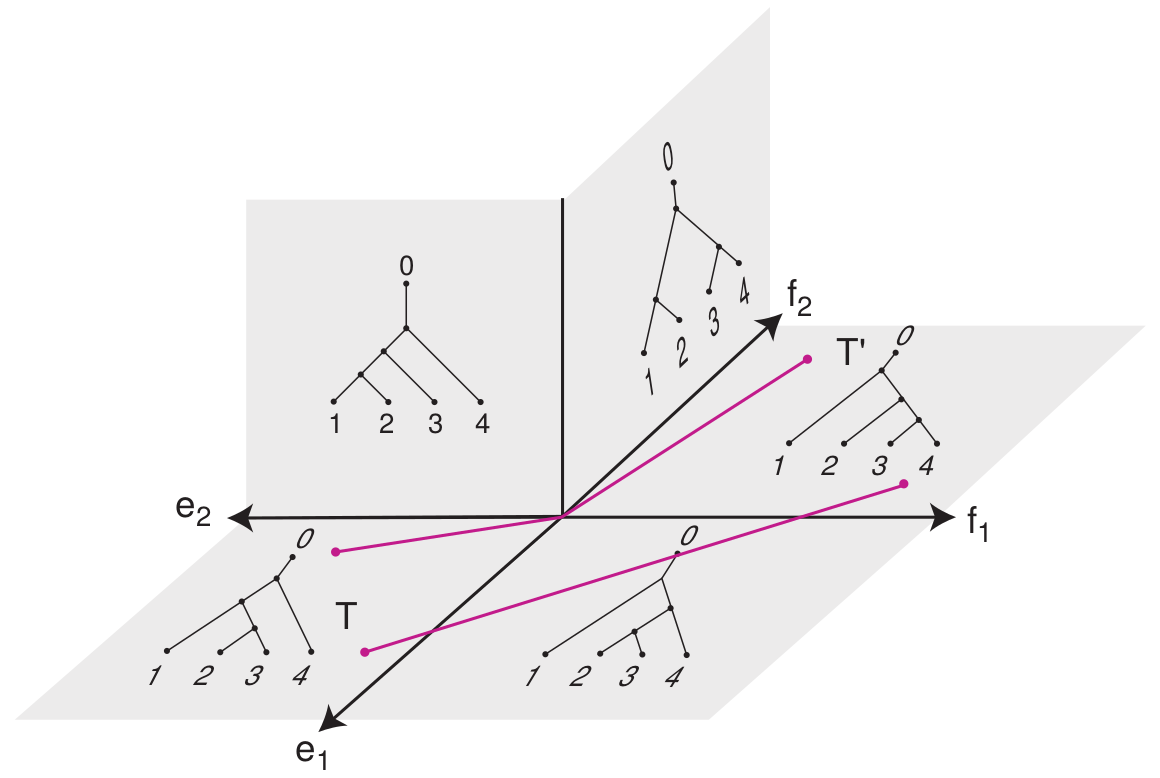
\includegraphics[width = 0.5\linewidth]{Figs/OrthantBHV-bis}
 \caption{Orthants in the BHV space of trees with 4 leaves and examples of two 
geodesics. As illustrated, the geodesics are not identical and therefore depend 
on both the topology and the actual branch lengths. Reproduced with 
permission from \citet{Billera2001}. Copyright 2001, Elsevier.}
\end{figure}

In Euclidean space, the Fr\'echet mean is the point minimizing the sum of the squared distances to the sample points, and is equivalent to the coordinate-wise average of the sample points. Similarly, the Fr\'echet mean tree is the tree minimizing the sum of squared BHV distances to a set of tree and that sum is the variance which quantifies how spread out the forest is \citep{miller2015polyhedral,brown2017mean}. \citet{Billera2001} showed that mean is unique and is not necessarily a refinement of the majority-rule consensus.

%%%%%%%%%%%%%%%%%%%%%%%%%%%%
\subsection{Use of BHV distance} \label{sec:means-and-variance}

BHV distances can be used in much the same way as euclidian distance and the standard tools of multivariate statistics can be used  to analyse the forest. For example, \citet{barden2014limiting} proved a Central Limit Theorem in the BHV space that can be used to either detect weakly and strongly supported edges in the mean tree or to test hypotheses on some portion of the tree. One of their main tool is the so-called log-map which projects the BHV metric space to the usual euclidian space and allows one to visualize the forest as a scatter plot to gain some understanding of the estimate uncertainty.

% \citet{barden2017logarithm} proved a Central Limit Theorem on the BHV treespace, showing that the distribution of the sample means converges to a certain Gaussian distribution. It is useful for detecting splits of weak and strong support and in tree-valued hypothesis testing.

% A key tool of \cite{barden2014limiting}is  the log map  that permits to  map  trees  from  their  metric  space  to  Euclidean space, where it is possible to model a tree estimate $\hat T$ as a noisy realization of the true tree $T$. Once  the model parameters are estimated, Euclidean multivariate analysis techniques to reduce the dimension of the trees can be used. This allows to visualize tree estimates, along with their uncertainties.

In the same spirit, \citet{willis2016confidence} use the distance matrix to
% For example it is possible to use the variance covariance matrix to
estimate  the  principal  directions  of  variability  via principal components analysis (PCA). The axes of the $\mathbb{R}^m$ ellipsoid indicate the relative directions of precision, and the ellipsoid can be shrunk  to be wholly contained in the same orthant as a focal tree $\hat{T}$. This gives an unambiguous indication of the relative confidence in the edges of $\hat{T}$. Note that the procedure is also explicit about the trees contained in the confidence set for a given confidence level $\alpha$. \citet{de2012phylo} use a similar approach based on a different mapping of the trees to a euclidian space and use multiple co-inertia analysis (MCOA) instead of PCA to detect the principal directions of variability.

Finally \citet{weyenberg2014kdetrees}  propose  a non-parametric estimator of the distribution that generated the forest $T_1,\ldots,T_n$.  This estimator can be viewed as a refined version of histogram-based estimation of a density. The kernel function, is a non-negative function defined on pairs of trees, which measures how similar two trees are. Kernel density estimation use the fact that points close to sample points tend to have higher likelihood than distant outlier points.  The ultimate goal is to detect outlier trees, $T_j$, which are not actually drawn from the true distribution.

% \cite{de2012phylo} developed a statistical non-parametric method to detect outlier trees from the set of gene trees. They first convert gene trees into vectors in a multidimensional Euclidean space and then apply multiple co-inertia analysis (MCOA)—an extension of principal coordinate analysis—directly to these vectorized gene trees. Their method, Phylo-MCOA, also detects outlier species, those whose position varies widely from tree to tree. Included in our results are simulation studies comparing our non-parametric method with Phylo-MCOA

%%%%%%%%%%%%%%%%%%%%%%%%%%%%
%\subsection{Confidence Sets Based on other Distances} \label{sec:kernel}
%
%Kernel based methods (using a distance matrix) to find outlier and build confidence sets.

%%%%%%%%%%%%%%%%%%%%%%%%%%%%
\subsection{Conclusion}

Nowadays efficient algorithms permit to compute means of continuous distances in a reasonable time. Moreover a huge amount of work has been done to derive mathematical properties of theses distances. Therefore it is possible to go from a theoretical work to applications. For example, \citet{Kendall2016} use tree mapping to show that 3 genes of Ebolavirus have markedly different phylogenies. This result is quite typical in genomic-scales analysis where different loci have different evolution history. This is a natural consequence of the gene trees / species tree problem whereby the evolutionary history of a gene can be different from the species tree \citep{Degnan2009}. This has spanned the entire research field of reconciliation devoted to the reconstruction of species tree from sets of gene tree. 

Distances between trees can help cluster trees and/or loci into congruent groups with the intent of performing one inference per group to infer more robust phylogenetic estimates. In an era of cheap and abundant sequences, tree validation is as much a matter of computing support values as a matter of validating and making sure there are not too many conflicting signals in the molecular data (taxa set, gene set) used for tree reconstruction. 